% TEMPLATE for Usenix papers, specifically to meet requirements of
%  USENIX '05
% originally a template for producing IEEE-format articles using LaTeX.
%   written by Matthew Ward, CS Department, Worcester Polytechnic Institute.
% adapted by David Beazley for his excellent SWIG paper in Proceedings,
%   Tcl 96
% turned into a smartass generic template by De Clarke, with thanks to
%   both the above pioneers
% use at your own risk.  Complaints to /dev/null.
% make it two column with no page numbering, default is 10 point

% Munged by Fred Douglis <douglis@research.att.com> 10/97 to separate
% the .sty file from the LaTeX source template, so that people can
% more easily include the .sty file into an existing document.  Also
% changed to more closely follow the style guidelines as represented
% by the Word sample file. 

% Note that since 2010, USENIX does not require endnotes. If you want
% foot of page notes, don't include the endnotes package in the 
% usepackage command, below.

% This version uses the latex2e styles, not the very ancient 2.09 stuff.
\documentclass[letterpaper,twocolumn,10pt]{article}
\usepackage{usenix,epsfig,endnotes}
\usepackage{tikz}
\usepackage{pgfplots}
\usepackage{url}
% Some maybe useful commands
\newcommand{\inlinecode}[1]{\texttt{#1}}

\begin{document}

%don't want date printed
\date{}

%make title bold and 14 pt font (Latex default is non-bold, 16 pt)
\title{\Large \bf Can RocketBufs Make an Impact?}

%for single author (just remove % characters)
\author{
{\rm Bryant Curto}\\
University of Waterloo
\and
{\rm Manoj Adhikari}\\
University of Waterloo
\and
{\rm Shahzaib Ali}\\
University of Waterloo
% copy the following lines to add more authors
% \and
% {\rm Name}\\
%Name Institution
} % end author

\maketitle

% Use the following at camera-ready time to suppress page numbers.
% Comment it out when you first submit the paper for review.
\thispagestyle{empty}


\subsection*{Abstract}
% P1: Abstract Intro:
%     -What is rocketbufs?(1 sentence)
%     -How it helps design better MOM systems(1 sentence)
% p2: Intro to our work:
%     - Reproduction study
%     - Multithreaded Redis
%     - Attempt to Utilize Rocketbufs with Redis
%     - Reviewing other works that improved MOM systems performance using RDMA
% P3: Results we found
%     1. Challenging to reproduce
%         - Required us to try out different number of producers to saturate the CPU
%         - 
%     2. Unfair comparisions through
%         - single threaded redis
%         - RBMQ Pipelining
%         - RBMQ no responses
%     3. Challenging to Adapt with Redis
    
RocketBufs is a framework for building high-performance, in-memory Message Oriented Middleware (MOM) systems produced by researchers from the University of Waterloo.
The authors claim that RocketBufs provides MOM developers access to modern data center networking technologies that can be easily utilized to increase performance.

%In this study, we review other works that utilize modern data center networking technologies to improve the performance of MOM systems.
In this study, we repeat the performance analysis conducted in the original paper.
%and show that RocketBufs may exhibit better performance than previously expected as compared to existing MOM systems.
Then, we discuss the challenges of adapting Redis, a popular industry grade MOM system, to run on top of RocketBufs.
This provides some insights into challenges for building or adapting other MOM systems to use RocketBufs.

Our work supports the argument that RocketBufs is a unique solution to an important problem. However, some hurdles exist that prevent it from being easily integrated into existing MOM systems.


\section{Introduction}
% 1. Current State of MOM Systems: how they transfer data
%     - What is MOM?
%     - Where it is used?
%     - How most MOM systems are used
% 2. What RocketBufs does
%     - Compares performance of Redis which uses TCP with the performance of RBMQ that uses RocketBufs (Both TCP and RDMA enabled)
%     - 
% 3. What Redis does
% 4. How other papers have modified Redis
% 5. What are the contributions of your paper?
% Terms to define for new readers:
% Client: No Need 
% Server: No need
% Publisher: A party that sends a message.
% Broker: A party that receives a message from publisher and sends to other brokers or subscribers.
% Subscriber: A party that receives a message.
% Socket: Not Needed
% Transport Protocol: Not Needed
% MOM Systems:  Message-Oriented Middleware or MOM
% provides a clean method of communication between disparate software entities. MOM is
% one of the cornerstone foundations that distributed enterprise systems are built upon. MOM
% can be defined as any middleware infrastructure that provides messaging capabilities\cite{curry2004message11}.
% Throughput: The amount of message transferred per time.
% Latency:
% NICs:  (NICs) are used by computer systems to enable them to communicate over networks with other computer systems. Commonly, NICs are available as plug in devices that are connected to a computer's interface bus (e.g., PCI Bus), or are built directly into a computer's mother board\cite{latif2002method12}.

Message-Oriented Middleware (MOM) systems provide a clean method of communication between disparate software entities.
Also referred to as publish/subscribe systems, they are any middleware infrastructure that provide messaging capabilities~\cite{curry2004message11}.
They are a popular class of software systems designed to support loosely-coupled
messaging in modern distributed applications~\cite{Rocketbufs}.
MOM systems are the foundation upon which modern distributed enterprise systems are built.
Companies that have high demands for message sharing can benefit from the improved performance of MOM systems.

One approach of improving the performance of MOM systems is to leverage modern and emerging data center networking technologies, especially those that offer kernel-bypass features to enable high-throughput and/or low latency communication such as Remote Direct Memory Access (RDMA)~\cite{RDMAOverTCP}.
%In the process of the conventional network transmission, data needs to be transferred
%and copied among user space, kernel space and network equipment. This entire
%transmission process involves the consumption of memory bandwidth and CPU cycles. However, the Remote Direct Memory Access (RDMA) technology allows the
%local host to directly access the remote host's application buffer without impacting the
%remote host's operating system~\cite{RDMAOverTCP}.
Similar to RDMA, there are other modern network communication technologies such as DPDK and TCPDirect which can significantly improve the performance of MOM systems. Most MOM systems use kernel-based TCP for communication and don't utilize modern data center networking technologies. This is because the API's and abstractions provided by each of these technologies are very different from TCP which makes them very challenging to adapt to.  

RocketBufs~\cite{Rocketbufs} is a framework designed to improve accessibility of modern and emerging networking technologies for MOM systems. It aims to assist developers in making use of these networking technologies and seamlessly switch between technologies as needed.

The claims of the RocketBufs paper regarding its performance and ease of use have not been evaluated by anyone other than the original authors.
We are the first to attempt a reproduction of their experiments.
We go beyond a reproduction to consider more real-world scenarios. In achieving this endeavor, we consider the challenges associated with adapting Redis, an industry grade MOM system, to use RocketBufs.

% LEAVE THIS DISCUSSION TO THE METHODOLOGY SECTION
%In addition, for our idea of adaptation, we assess the original implementation of MOM system, RBMQ (Rocketbufs Message Queueing), that uses Rocketbufs as an underlying framework. We use the original artifacts to make an attempt in reproducing the results of the paper. The hardware specifications as well as the testbed used for the reproduction are the same as described in the experimental setup of the paper. To our knowledge, the configurations of certain aspects of the experiments that are not explicitly mentioned in the original paper are deduced from the information in the paper. One such example is the saturation of broker with multiple producers, which we replicate by running multiple producer instances on client machines to produce a large number of messages.

Through our work, we make the following contributions:
\begin{enumerate}
\item We reproduce a subset of the performance analysis conducted in the RocketBufs research paper. We evaluate the performance of RBMQ, a proof-of-concept MOM system built on top of RocketBufs, using TCP.
%First, the paper claims that RBMQ which is implemented using RocketBufs provides better throughput than Redis and RabbitMQ . We tested this claim for TCP-enabled Rocketbufs by reproducing the experiments and remeasuring throughputs. 

\item We discuss the challenges faced in building or adapting an MOM system to run on top of RocketBufs by considering the challenges in adapting Redis, an industry grade MOM system.
%Second, the paper argues that RocketBufs is easily adaptable to industry grade applications such as Redis. We modified Redis to use RocketBufs in an attempt to transfer data between publishers and brokers. We did not have enough time to use RocketBufs between brokers and subscribers and our experience doesn't support the claim that RocketBufs is easily adaptable.
\end{enumerate}



\section{Background and Related Work}
%This section provides an overview of the topics at hand. Further, it discusses what work has been conducted on this topic and how our work stands out.

\subsection{Background}
% Question: What is an MOM application?
% This is to give the reader an idea of the topic at hand before jumping into RocketBufs
% This is also to set up the problem that RocketBufs solves
% From the RocketBufs paper:
%   - "Unfortunately, commonly-used MOM systems do not take advantage of these ca- pabilities and instead use kernel-based TCP, which in many cases incurs protocol processing and copying overhead (even for com- munication within a data center [27]), limiting throughput and resulting in higher latency. One reason current MOM systems avoid using emerging tech- nologies is the complexity of supporting multiple communication substrates in a single MOM implementation. For instance, the native RDMA verb interface uses abstractions and APIs fundamentally different from the socket abstraction that are quite complicated to use~\cite{RDMAOverTCP}. As a result, significant engineering effort would be required for both new and existing MOM systems to support RDMA and TCP, since two separate data transfer implementations would be re- quired. Similarly, emerging technologies often initially provide new abstractions and custom APIs that require additional modifications to the MOM system implementation (e.g., DPDK [69])."



% Question: What is RocketBufs?
A Message-Oriented-Middleware (MOM) System is any middleware infrastructure that provides messaging capabilities.
A client of an MOM system can send messages to, and receive messages from, other clients of the messaging system with one or more servers acting as intermediaries in message delivery~\cite{doi:https://doi.org/10.1002/0470862084.ch1}.
We refer to sending clients as publishers, receiving clients as subscribers, and intermediary servers as brokers.

RocketBufs is a framework which provides infrastructure for building high-performance, in-memory MOM systems. It provides memory-based buffer abstractions and APIs designed to work efficiently with different network communication technologies (e.g., TCP and RDMA).
It offers MOM system developers easy access to modern network communication technologies~\cite{Rocketbufs}, and thereby any performance improvements that come about through use of these technologies.
% How does RocketBufs solve this problem?
% From the RocketBufs paper:
%   - "By de- signing abstractions and APIs that work well with both RDMA and TCP, two protocols with vastly different programming interfaces, we believe that other transport layer APIs and technologies like QUIC [31], DPDK [69], F-Stack [21], and Solarflare/TCPDirect [64] could also be efficiently supported by the framework, providing benefits to all applications built using RocketBufs."
% Connect RocketBufs to Redis
In the original RocketBufs paper, a publish-subscribe message queuing system named RocketBufs Message Queue (RBMQ) is implemented using RocketBufs and its performance is compared with a popular MOM system called Redis.

%What is Redis?
Redis is a widely used, production quality, in-memory data structure store that can be used as an MOM System~\cite{redis-intro}. Companies like Engine Yard, Github, Craigslist, Disqus, Digg, and Blizard are part of the growing list of Redis adopters~\cite{macedo2011redis6}.

%Might be avoid mentioning this entirely
%RabbitMQ is another well-known MOM system. It is used by companies such as Reddit, Robinhood, and Accenture\cite{stackshare7}.
%Hoang et al. show that RBMQ has throughput comparable to or slightly lower than that of Redis when using TCP with flow control enabled. They also perform experiments by disabling flow control to measure the throughput without buffer synchronization overhead.
%In addition, this setup is more comparable with Redis which also doesn't have flow control.
%In addition, they show that when RDMA is enabled for RBMQ, the system's performance is nearly double that of Redis under all sets of conditions for messages sizes 8 bytes to 2K bytes, inclusive.
%The results of this performance evaluation can be seen in Figure \ref{fig:TODO}.

% While the following is true, but I feel like it's kind of obvious:
%However, to fully understand the complexity of using RocketBufs with other MOM systems than Redis, each implementation needs to be considered separately.


\subsection{Related Work}

% How does RocketBufs stand out?
% Also, I think that this should be moved to the top of the Related Work Section
\subsubsection{Networking Technology Libraries}
Numerous APIs are available to MOM system developers that can be used to take advantage of modern networking technologies.

Libraries such as rsocket and libfabric provide new APIs and access to modern networking technologies such as RDMA. Further, they attempt to perform RDMA-based optimizations~\cite{Rocketbufs}.
However, these solutions do not provide a comparable framework to RocketBufs.

% Briefly, why are they inferior to RocketBufs
Mellanox's Messaging Accelerator (VMA) requires no application change because it provides standard socket TCP, UDP (Unicast, Multicast) to the application layer. In addition it enables Kernel bypass which reduces kernel overhead by creating direct application to network adapter access. It purports benefits such as lower latency, higher throughput, and lower CPU utilization~\cite{mellanox9}. However, this solution also doesn't provide a comparable framework to RocketBufs and doesn't enable the ability to easily switch to a different data center networking technology.

%Need to write how this solution is different from RocketBufs
The key differences between other libraries and RocketBufs is that RocketBufs provides a middleware with much higher level APIs and abstractions that are designed to naturally and explicitly support the building of a wide range of efficient message-oriented systems. We could find no other frameworks that allow applications to utilize modern data center networking technologies and permit the transition to another networking technology with no alterations to application code.


\subsubsection{Redis Network Communication}
%What work is similar? (RDMA Papers)
Redis has previously been adapted to utilize modern data center networking technologies.

Tang et al. show that adapting Redis to use RDMA instead of TCP sockets can improve performance by increasing throughput, reducing latency and reducing CPU utilization~\cite{RDMAOverTCP}. 
%How is this similar and different?
%The objectives of our work is very similar to this paper because we would also be measuring performance of RDMA enabled Redis.
%Similar
%Different
However, since Redis is adapted directly to make use of RDMA, taking advantage of a different networking technology (e.g., DPDK) would require a completely new implementation. In contrast, once RocketBufs is able to support a new networking technology, any MOM system developer wishing to make use of the new technology need to only change a configuration file.

Qi et al. design a high performance Redis system by replacing the traditional Unix socket interface with Fast Event Driven RDMA RPCs (FeRR)~\cite{RediswithRPCs5}.
%How is this similar and different?
The authors make additional modifications to Redis such as optimizing the Redis serialization protocol. Further, they replace Redis' single thread framework with a parallel task engine. These additional modification to Redis make it difficult to distinguish what benefits were gained through using RDMA and what benefits were due to other changes. This paper similarly focuses on adapting Redis to use RDMA directly and suffers from the same inability to adapt to other networking technologies.

%How's our work different from them?

\section{Experimental Setup}
%This section explains ...TODO... the hardware and software setup that we used in order to reproduce original experiments. 
% this section explains


\subsection{Hardware}
The hardware for our performance evaluation is comprised of a cluster of thirteen machines.
The machine running the broker contains an Intel Xeon E5-2660 v3 CPU with 10 cores clocked at 2.60GHz and 512 GBs of RAM.  We call this machine the broker machine.
The remaining twelve machines in the cluster are used to run clients (i.e., publishers or subscribers) and are called client machines.
These machines contain an Intel Xeon CPU D-1540 with 8 cores clocked at 2.00 GHz and 64 GB of RAM.
Four 40 Gbps NICs are configured on the broker machine to connect to 4 mutually exclusive subsets of client machines in the cluster connected via their own single 40 Gbps NIC.
As a result, the broker has up to 160 Gbps of bi-directional bandwidth available to communicate with clients.
Each subset is configured to communicate over an exclusive network.
By designating each subset of machines be used for either publishers or subscribers, we avoid publisher and subscriber messages interfering with one another.
We did not saturate the NICs for any of our experiments.
%in order to avoid on a different subnet. The client host machines  all have the same hardware specifications with , and a single 40 Gbps NIC. In addition, we used a machine used for publishers with Intel Xeon CPU E5-2697 v3 with 28 cores each clocked at 2.60GHz, 264 GB of RAM, and six 40 Gbps NICs but we only use one. We used the broker host machine for both Redis and RBMQ as it has 160 Gbps of bi-directional bandwidth available for accepting connections from both the subscribers and the publishers.
All machines run Ubuntu 18.04.1 with Linux kernel version 4.18.0.

Note that the hardware specifications are nearly identical to those used in the original performance evaluation of RBMQ~\cite{Rocketbufs,hoang2019building} with the exception of OS version (Ubuntu 18.04.2).
As a result, we expect similar results.


\subsection{Setup}
\subsubsection{Redis}
In our evaluation, we use Redis version 6.0.9.
Each Redis publisher instance spawns ten threads, each of which continuously publishes messages to one of ten topics.
Redis uses a Request/Response Protocol~\cite{redis-req-resp}.
As a result, each publisher thread publishes a message to a topic by submitting the message to the Redis broker, waiting for acknowledgement, and then submitting the next message.

Each Redis subscriber instance spawns ten threads such that each thread subscribes to a single topic.
Once subscribed, each subscriber thread simply counts the number of messages it receives from the broker.
We compare RBMQ with Redis instead of another MOM system (e.g., RabbitMQ) because of the similarity in throughputs of the systems reported in the RocketBufs paper.

\subsubsection{RBMQ}
Each RBMQ publisher instance spawns a multiple of ten threads, each of which continuously publishes messages using it's own personal RocketBufs buffer.
RBMQ does not use a Request/Response Protocol. Publishers handle responses from the broker asynchronously.
As a result, we configured publishers to publish messages at a constant rate of 50,000 messages per second, which we found to be consistent with Redis on average for our selected message sizes.

Each RBMQ subscriber instance spawns ten threads such that each thread subscribes to a non-overlapping subset of RocketBufs buffers to which messages are published.
Once subscribed, each subscriber thread simply counts the number of messages it receives from the broker.


\section{Evaluation}
%This section presents our results from reproducing the performance analysis of RMBQ using TCP with flow control enabled and Redis.

\subsection{Methodology}
% Please read over the reproduction paper the Professor Brecht posted: https://dl.acm.org/doi/pdf/10.1145/3402413.3402418
% I think this section is too narrative in nature.
% leave this for now though
Originally, four different types of RBMQ experiments are performed. These experiments vary in the transport protocol configurations that they use. These transport protocol configurations include client and broker both communicating via TCP with flow control enabled (RBMQ-tcp-tcp), via TCP with flow control disabled (RBMQ-tcp-no-fc), and via RDMA (RBMQ-rdma-rdma). The final configuration is publisher and broker communicating via TCP while broker and subscriber communicate via RDMA (RBMQ-tcp-rdma).
In our reproduction, we evaluate the performance of RBMQ with clients communicating with the broker using TCP with flow control enabled (RBMQ-tcp-tcp).
We do not evaluate the performance of RBMQ using TCP with flow control disabled (RBMQ-tcp-no-fc) because it is only used as a means of understanding the overhead of flow control~\cite{hoang2019building}.
%"Note that, this configuration may not be useful for delivering messages in real-world pub/sub systems, because it could result in buffer data being overwritten by the framework. We include it as a theoretical point of comparison in order to understand the overhead of flow control."
Further, we do not evaluate the performance of RBMQ using RDMA (RBMQ-rdma-rdma and RBMQ-tcp-rdma) because it would be more difficult to compare both systems as Redis does not natively support use of RDMA.
Most importantly, RBMQ using TCP with flow control enabled offers the most straight forward method of comparing performance as Redis uses TCP.

In our experiments, we use separate hosts for broker, publisher, and subscriber instances. Each publisher instance uses multiple threads to produce messages of a fixed size. Each subscriber instance subscribes to all publisher topics, thereby consuming all data produced by the publishers.



%For RabbitMQ, we use the rabbitmq-c client library [13] to implement the publishers and subscribers. RabbitMQ offers an option where subscribers send an acknowledgement message to the broker upon receiving a message. This option allows the broker to inform the publisher about the completion of message delivery, however it incurs extra commu- nication costs compared to Redis and RBMQ which do not implement this feature. We therefore disable it in all of our experiments for a fair comparison. Our Redis publishers and subscribers are implemented using the Redis-provided client library hiredis [83]. We run multiple Redis broker processes on the broker host in order to utilize all CPU cores, since each Redis broker process is single-threaded. For both Redis and RabbitMQ, we disable data persistence and event logging features to ensure that messages are handled in-memory only. We also tune both systems based on recommended best practices [78, 86] to optimize their messaging performance in our experiments.
%The message broker processes run on a host containing a 2.6 GHz Intel Xeon E5-2660v3 CPU with 10 cores, 512GB of RAM, and four 40Gbps NICs for a total of 160Gbps bidirectional bandwidth (we refer to this hardware as a “big host”). Subscribers and publishers run on separate hosts which contain a single 2.0 GHz Intel Xeon D-1540 CPU with eight cores, 64 GB of RAM, and a single 40 Gbps NIC (we refer to this hardware as a “regular host”). We benchmarked our NICs using iPerf [52] and found that the maximum throughput they can achieve is 38Gbps. All nodes run Ubuntu 18.04.2 with a version 4.18.0 Linux kernel. To avoid network contention, each subscriber connects to a separate NIC on the host running the broker. Each experiment is run for 150 seconds, with data being collected during the 120 second steady-state period following a 30 second warmup period. The experimental results are reported with 95% confidence intervals, except for the latency experiments where the data points are reported as CDFs. Note that, the confidence intervals are typically small relative to the sizes of the data points, and therefore in most cases they are not visible on the graphs.
%When running experiments on a system using multiple CPU cores and NICs, we find that tuning the interrupt request queues (IRQ) of network devices is also important for performance. Our IRQ tuning includes: disabling the Linux irqbalance daemon (which is enabled by default in most current Linux distributions); and binding each device queue to a single CPU core, while distributing the number of device queues evenly among cores (note that a network interface can have multiple queues). This ensures that interrupts generated by a queue are handled by the same CPU core, while also allowing all cores to be used for interrupt handling.
%In this experiment, we measure the maximum message throughput that can be achieved by a message broker host in terms of number of messages delivered per second (mps). We configure the publishers to constantly send messages to the broker by calling the publish function in a tight loop. To find the maximum throughput values, we increase the number of publisher threads (and therefore the number of topics) until the throughput stops increasing. This corresponds to the point at which, depending on the experiment, either the broker node’s CPU is close to 100% utilization or the NIC is saturated. In our experiments, we find that using up to 20 publisher threads (running on one or more hosts depending on the experiment) allows all target systems to reach these points. Additionally, for this experiment, we also benchmark RBMQ using TCP (for all communication) with flow control disabled (denoted as RB-tcp-no-fc). Note that, this configuration may not be useful for delivering messages in real-world pub/sub systems, because it could result in buffer data being overwritten by the framework. We include it as a theoretical point of comparison in order to understand the overhead of flow control.

Prior to performing our experiments, we follow the steps described in the original evaluation~\cite{Rocketbufs,hoang2019building}.
We disable the Linux irqbalance daemon, which is enabled by default in most current Linux distributions.
Further, we disable hyperthreading on each machine to ensure that our measurements are not negatively influenced by threads running on the same physical core.
Each experiment is run for a minimum of 150 seconds where data is collected for only the latter 120 seconds.
This is to avoid variability caused by experiment initialization from influencing our results.

%In contrast to Hoang's thesis, we did not
%- binding each device queue to a single CPU core, while distributing the number of device queues evenly among cores (note that a network interface can have multiple queues). This ensures that interrupts generated by a queue are handled by the same CPU core, while also allowing all cores to be used for interrupt handling.
%- we used far more than 20 publisher threads

During our evaluation, we found our measurements to be highly sensitive to the number of publisher processes used.
Using too few publishers results in the broker's resources not being saturated. However, using too many publishers can result in overhead from message buffering and flow control.
In order to determine the optimal number of publishers, we first run the experiment with a sufficient number of publishers to saturate the cores of the broker's machine.
We then rerun the experiment, performing a binary search of the possible number of publishers until arriving at the number of publishers for which we observed best throughput.


%\subsection{Reproducing the Experiments}
%To reproduce the experiments, we started by looking into RocketBufs source code. First, we discovered that the RBMQ evaluation code lies inside the \verb|rbuf_eval| directories that are inside the \verb|/include| and \verb|/src| directories of \verb|/kappa| directory. We noticed that the \verb|/include| directory contains the header files, while the \verb|/src| directory has the main code. Further inspecting the main function, we saw that the client or broker is started by passing a set of flags that are defined in \verb|eval_common.hpp.| \\

%Need to finish reformating so that this looks good
%To run the broker process, we can run it as follows: 
%\begin{verbatim}
%/rbuf_eval b –p 1 –c 1 –b 1 –a <broker-adress> -d <broker-port> -r false
%\end{verbatim}
% (and similarly rest of the arguments)

%After the broker is up and running, we can run the producer on another machine as follows: 

%\verb|./rbuf_eval (c or p) –a <broker-address> -d <broker-port> -e <client-address> -u <client-port> |

%(c or p) -> run client as either consumer or producer 


\begin{figure}[!t]
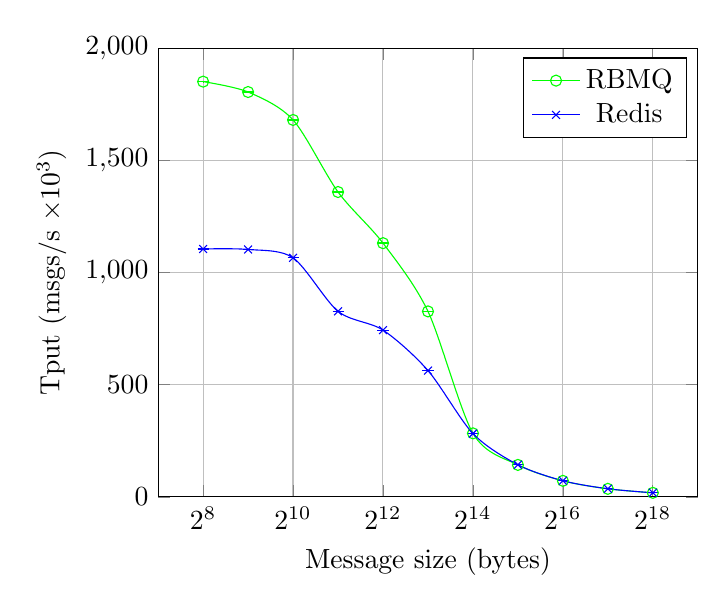
\begin{tikzpicture}
    \begin{axis}[
        xlabel=Message size (bytes),
        ylabel=Tput (msgs/s $\times 10^3$),
        ymin=0, ymax=2000,
        xmode=log, log basis x=2,
        enlarge x limits={0.1},
        grid=both,
%        xticklabel = {
%            \pgfmathparse{\tick/1000}
%            \pgfmathprintnumber{\pgfmathresult}\,K
%        }
    ],
        % $10^3)$
%\iffalse
%    \addplot[smooth,color=red,mark=x, error bars/.cd, y dir=both, y explicit]
%        plot coordinates {
%        (2^8,837.024083333333)+=(0,37.62921125)-=(0,37.62921125)
%        (2^9,760.9649833333331)+=(0,25.1731309)-=(0,25.1731309)
%        (2^10,677.570841666666)+=(0,27.58022904)-=(0,27.58022904)
%        (2^11,649.117658333333)+=(0,19.927291519999997)-=(0,19.927291519999997)
%        (2^12,1022.17253333333)+=(0,56.619253539999995)-=(0,56.619253539999995)
%        (2^13,543.6213583333331)+=(0,18.198130539999998)-=(0,18.198130539999998)
%        (2^14,277.52054166666596)+=(0,5.680146692999999)-=(0,5.680146692999999)
%        (2^15,140.415758333333)+=(0,1.3285205960000002)-=(0,1.3285205960000002)
%        (2^16,70.733675)+=(0,0.3050638536)-=(0,0.3050638536)
%        (2^17,35.4617916666666)+=(0,0.08503276571000001)-=(0,0.08503276571000001)
%        (2^18,17.7626666666666)+=(0,0.009913312746)-=(0,0.009913312746)
%        
%        };
%    \addlegendentry{RBMQ}
%\fi
        \addplot[smooth,color=green,mark=o, error bars/.cd, y dir=both, y explicit]
        plot coordinates {
            (2^8,1852.22149)+=(0,1.1630446492476634304)-=(0,1.1630446492476634304)
            (2^9,1805.85814)+=(0,1.2356001885343979858)-=(0,1.2356001885343979858)
            (2^10,1681.26714)+=(0,0.79848911099077919085)-=(0,0.79848911099077919085)
            (2^11,1359.7994199999998)+=(0,1.077124544)-=(0,1.077114544)
            (2^12,1131.60194)+=(0,2.3586789290000003)-=(0,2.3586755950000002)
            (2^13,827.18456666666666666)+=(0,0.25259628441008466271)-=(0,0.25259628441008466271)
            (2^14,283.16284166666666667)+=(0,0.019044062828730686798)-=(0,0.019044062828730686798)
            (2^15,142.41825)+=(0,0.009362639644512926184)-=(0,0.009362639644512926184)
            (2^16,71.289333333333333336)+=(0,0.0037207963290730902341)-=(0,0.0037207963290730902341)
            (2^17,35.654408333333333335)+=(0,0.0017483522426190725986)-=(0,0.0017483522426190725986)
            (2^18,17.810166666666666666)+=(0,0.0010706164081828917358)-=(0,0.0010706164081828917358)
        };
    \addlegendentry{RBMQ}
    \addplot[smooth,color=blue,mark=x, error bars/.cd, y dir=both, y explicit]
        plot coordinates {
         (2^8,1105.70206666666)+=(0,0.2439285709)-=(0,0.2439285709)
        (2^9,1103.5177166666601)+=(0,0.2075071549)-=(0,0.2075071549)
        (2^10,1066.0545)+=(0,0.1960125185)-=(0,0.1960125185)
        (2^11,827.624166666666)+=(0,0.30654419130000005)-=(0,0.30654419130000005)
        (2^12,743.795133333333)+=(0,0.1300893028)-=(0,0.1300893028)
        (2^13,563.29175)+=(0,0.026386139700000002)-=(0,0.026386139700000002)
        (2^14,282.208183333333)+=(0,0.01938056605)-=(0,0.01938056605)
        (2^15,143.080283333333)+=(0,0.007250361859)-=(0,0.007250361859)
        (2^16,71.64473333333329)+=(0,0.004665160073)-=(0,0.004665160073)
        (2^17,35.9301333333333)+=(0,0.002134183088)-=(0,0.002134183088)
        (2^18,17.9738166666666)+=(0,0.0014732622319999999)-=(0,0.0014732622319999999)
        };
    \addlegendentry{Redis}
    \end{axis}
    \end{tikzpicture}
    \caption{Throughput of RBMQ and Redis with zero subscribers and 95\% confidence intervals.}
    \label{fig:0sub}
\end{figure}

\subsection{Throughput with 0 Subscribers}
Figure \ref{fig:0sub} plots the maximum throughput of messages that can be processed by the Redis and RBMQ brokers with no subscribers.
In this experiment, publishers send messages to the broker which are immediately discarded.
The plot also includes 95\% confidence intervals, which are difficult to see as a result of their size.
This experiment serves as a means of understanding how our experimental setup compares to that of the original.

The figure shows that RBMQ performs noticeably better than Redis for message sizes in range $2^{8}$ to $2^{13}$ bytes.
For message sizes of $2^8$ bytes, RBMQ's throughput is approximately 67\% greater than that of Redis.
For message sizes in range $2^{14}$ to $2^{18}$ bytes, the performance of RBMQ and Redis is nearly identical.

Comparing our findings with those presented in the RocketBufs paper~\cite{Rocketbufs} and Hoang's thesis~\cite{hoang2019building}, we take note of three key things.
First, our measurement of Redis' throughput is almost identical to that presented in the previous evaluation.
Second, our measurement of RBMQ's throughputs for messages of size $2^8$ to $2^{13}$ bytes is much higher than those originally observed.
In the original evaluation, this version of RBMQ is reported to have a maximum throughput of approximately 900 thousand messages per second for messages of size $2^8$ and $2^9$ bytes.
The throughput then drops as low as approximately 750 thousand messages per second for messages of size $2^{12}$ bytes.
For messages of size $2^8$ bytes, we measure RBMQ's throughput to be over 1.85 million messages per second, which is over double that originally measured.
Third, for message sizes in range $2^{14}$ to $2^{19}$, our throughput measurement of RBMQ is nearly identical to that presented in the original evaluation.

In the original evaluation, the number of publisher threads are steadily increased until the throughput stopped increasing.
At most 20 publisher threads are used to saturate the broker.
We believe that our approach in determining the optimal number of publishers to fully saturate the broker for messages of a given size (previously described) enables us to eke out additional performance from the RBMQ broker.

%We configure the publishers to constantly send messages to the broker by calling the publish function in a tight loop. To find the maximum throughput values, we increase the number of publisher threads (and therefore the number of topics) until the throughput stops increasing. This corresponds to the point at which, depending on the experiment, either the broker node’s CPU is close to 100% utilization or the NIC is saturated.
%In our experiments, we find that using up to 20 publisher threads (running on one or more hosts depending on the experiment) allows all target systems to reach these points.

%In the zero-subscriber benchmarks (Figure 5a and 5b), messages published to the broker are not forwarded to any subscriber and are discarded immediately. These benchmarks allow us to obtain insights about the ingest capacity of the broker and the cost of dis- seminating data to subscribers.


\begin{figure}[!t]
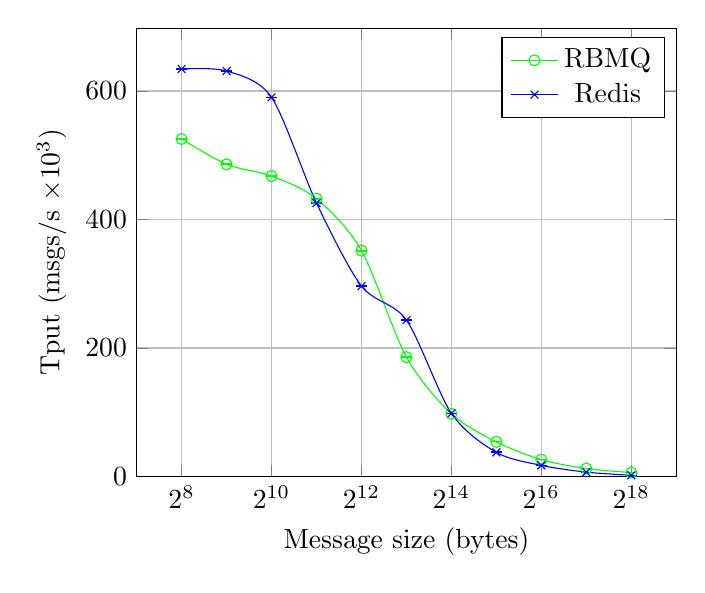
\begin{tikzpicture}
    \begin{axis}[
        xlabel=Message size (bytes),
        ylabel=Tput (msgs/s $\times 10^3$),
        ymin=0,
        xmode=log, log basis x=2,
        enlarge x limits={0.1},
        grid=both,
    ]

% BELOW PLOT COMMENTED OUT
\iffalse
    \addplot[smooth,color=black,mark=x, error bars/.cd, y dir=both, y explicit]
        plot coordinates {
            (2^9,947.1136)+=(0,1.135396735)-=(0,1.135263402)
            (2^10,994.8811)+=(0,0.115219001)-=(0,0.115219001)
            (2^11,701.5382)+=(0,0.2089640766)-=(0,0.2088640766)
            (2^12,694.2223)+=(0,0.2195602564)-=(0,0.2193935898)
            (2^13,323.4053)+=(0,0.2503490371)-=(0,0.2502490371)
            (2^14,174.7391)+=(0,0.5610965200000001)-=(0,0.5610298533)
            (2^15,85.53956)+=(0,0.377931034)-=(0,0.3779177007)
            (2^16,32.3421)+=(0,0.05929373536)-=(0,0.05929373536)
            (2^17,10.44086)+=(0,0.03843512896)-=(0,0.03842179562)

        };
        \addlegendentry{Redis}
        \addplot[smooth,color=red,mark=x, error bars/.cd, y dir=both, y explicit]
        plot coordinates {
            (2^8,513.6452)+=(0,0.5476624498999999)-=(0,0.5475957833)
            (2^9,485.75840000000005)+=(0,0.48550138179999996)-=(0,0.48550138179999996)
            (2^10,467.6197)+=(0,0.4066491125)-=(0,0.4066324458)
            (2^11,432.4169)+=(0,0.5830411291)-=(0,0.5830077958000001)
            (2^12,351.4819)+=(0,0.5822159391)-=(0,0.5820992724)
            (2^13,185.82)+=(0,0.4329199924)-=(0,0.4327866591)
            (2^14,97.60411)+=(0,0.10551726659999999)-=(0,0.1055039333)
            (2^15,54.03898)+=(0,0.05422673322)-=(0,0.05422006655)
            (2^16,26.30753)+=(0,0.03157549308)-=(0,0.03156882641)
            (2^17,12.47289)+=(0,0.01500661753)-=(0,0.0150032842)
            (2^18,6.20995)+=(0,0.0113707724)-=(0,0.0113707724)
        };
    \addlegendentry{RBMQ Publisher}
\fi

    \addplot[smooth,color=green,mark=o, error bars/.cd, y dir=both, y explicit]
        plot coordinates {
            (2^8,525.28965)+=(0,0.43278847985785823455)-=(0,0.43278847985785823455)
            (2^9,485.823)+=(0,0.4829295456)-=(0,0.48287954559999996)
            (2^10,467.58979999999997)+=(0,0.37889251789999995)-=(0,0.3787925179)
            (2^11,432.40979999999996)+=(0,0.2960604871)-=(0,0.2958938204)
            (2^12,351.5146)+=(0,0.5670100402)-=(0,0.5669767068999999)
            (2^13,185.7915)+=(0,0.4200196067)-=(0,0.4199696067)
            (2^14,97.60255000000001)+=(0,0.09336207281)-=(0,0.09334540615)
            (2^15,54.039410000000004)+=(0,0.050206557510000006)-=(0,0.05019322417)
            (2^16,26.30731)+=(0,0.02623213269)-=(0,0.02621879936)
            (2^17,12.471950000000001)+=(0,0.01226899144)-=(0,0.01225232478)
            (2^18,6.2106)+=(0,0.01205749591)-=(0,0.01205749591)

        };
    \addlegendentry{RBMQ}
    
        \addplot[smooth,color=blue,mark=x, error bars/.cd, y dir=both, y explicit]
        plot coordinates {
            (2^8,634.12165)+=(0,0.07412641813253469)-=(0,0.07412641813253469)
            (2^9,631.0123333333333333)+=(0,0.16584900025912221284)-=(0,0.16584900025912221284)
            (2^10,589.96968333333333334)+=(0,0.10391143324930754983)-=(0,0.10391143324930754983)
            (2^11,425.60941666666666666)+=(0,0.10206145129126576153)-=(0,0.10206145129126576153)
            (2^12,296.39035)+=(0,0.75166904255183064437)-=(0,0.75166904255183064437)
            (2^13,243.43763333333303)+=(0,0.23271337431087902)-=(0,0.23271337431087902)
            (2^14,98.30368333333333333)+=(0,0.09571882038126067333)-=(0,0.09571882038126067333)
            (2^15,37.635400000000004)+=(0,0.6329006426578839)-=(0,0.6329006426578839)
            (2^16,17.39275)+=(0,0.1647627131957749553)-=(0,0.1647627131957749553)
            (2^17,6.88145)+=(0,0.04299591526796371461)-=(0,0.04299591526796371461)
            (2^18, 1.9553833333333333333)+=(0,0.031833823881092294989)-=(0,0.031833823881092294989)
        };
    \addlegendentry{Redis}
    \end{axis}
    \end{tikzpicture}
    \caption{Throughput of RBMQ and Redis with one subscriber and 95\% confidence intervals.}
    \label{fig:1sub}
\end{figure}

\subsection{Throughput with 1 Subscribers}
Figure \ref{fig:1sub} plots the maximum throughput of messages delivered by the Redis and RBMQ broker to a single subscriber.
The figure also includes 95\% confidence intervals, which are difficult to see as a result of their size.

The figure shows that Redis performs better than RBMQ for messages of size in range $2^8$ to $2^{10}$ bytes.
RBMQ's throughput is as much as 23\% lower than that of Redis for messages of size $2^{9}$ bytes.
For messages of size $2^{11}$ bytes and larger, Redis and RBMQ perform similarly except for messages of size $2^{12}$ bytes and $2^{13}$ bytes.
For the prior, RBMQ has a throughput of approximately 19\% higher than that of Redis.
For the latter, RBMQ has a throughput of approximately 24\% lower.

Comparing our findings to those presented in Hoang's thesis~\cite{hoang2019building}, we note the following.
First, our measured performance of Redis is noticeably higher for messages of size $2^{8}$ to $2^{10}$ bytes.
The throughput is originally reported to be approximately 500 thousand messages per second for this range of message sizes.
In both evaluations, throughput is approximately the same for messages of size $2^{11}$ bytes.
Second, for values from $2^{12}$ to $2^{18}$ bytes, we observe a drop in Redis' throughput ranging from approximately 30\% for the smaller message sizes and 70\% for the larger when compared to the original evaluation of Redis.
Third, we measure the performance of RBMQ to be higher for messages of size $2^{8}$ to $2^{11}$ bytes by up to 30\% compared with the original evaluation of RBMQ.
Forth, for messages of size $2^{12}$ bytes, we observe similar throughput of RBMQ, but observe a decrease in throughput of up to 75\% percent for message sizes in range $2^{13}$ to $2^{18}$ bytes.
%75% for 2^15 msg size 150 and 37

As before, we believe that some of the disagreement with the findings in the original study may be attributed to the method we used to determine the number of publishers.
Further, we think that differences could have been caused due to a different Redis version being used in the original evaluation (the version is not specified).
%There may be other unknown variables with our experimental setup which gave us different results from original experiments.
To our knowledge, our setup and hardware is nearly identical to that described in the original paper.
As a result, we would expect to observe nearly identical results.

%Another possibility is that the original experiments were reported incorrectly. If the authors added multiple repetitions of their experiments to confirm that they got similar result in different trials, the value of this interpretation could have been weakened. We run multiple trials for each experiment in a similar setup and got very different throughput values. From the Rocketbufs paper and the thesis, it is unclear if this variability between trials exists during original experiments. 

%I am not sure if this statement is true, based on the differences that we showed on the graphs. For example, for 2^15 1 subscriber RBMQ
The pattern in our measured throughput for Redis and RBMQ is similar to that in the original study for larger message sizes but the measured values are different.
This suggests that our experimental setup differed from that of the original in one or more ways resulting in lower observed throughputs.
%Overall, we believe that the primary cause of these discrepancies is a result of a lack of experimental artifacts of the original evaluation.


\subsection{Assumptions}
In performing a reproduction of this work, we make several assumptions due to the lack of experimental artifacts.

The RBMQ subscriber should be run using 10 threads.
From the available code, we were able to infer that Redis subscribers utilized ten threads for handling messages from the broker.
As a result, we made the assumption that the RBMQ subscriber should use the same (Figure \ref{fig:1sub} shows results using this setup).
In order to validate this assumption, we measured the throughput for a number of message sizes where the RBMQ subscriber made use of only one thread.
However, we found that this change resulted in the subscriber becoming a bottleneck such that, no matter the number of publishers, we were not able to saturate the broker.

Only one RBMQ broker should be run on the broker machine.
We determined that the number of brokers must be at least equal to the number of subscribers.
However, we were not able to determine how more or fewer brokers would affect the evaluation.

The RBMQ broker should send responses to the publisher after each message is successfully published.
This option is disabled by default in RBMQ.
However, Redis follows a Request/Response Protocol~\cite{redis-req-resp}.
Leaving this option disabled would result in a weakening of the comparison of the two broker systems.

The Redis broker is composed of ten distinct, non-communicating Redis server instances, which was determined from the experimental artifacts and feedback from Hoang.
We validate this setup in our benchmark with zero subscribers (see Figure \ref{fig:0sub}).
However, this setup appears unrealistic as the lack of communication between the Redis instances results in no coordination between instances. This configuration may not serve as a valid comparison for RBMQ.
Without the overhead of coordination, measured throughputs of the Redis broker would be higher.
To validate this, we create a Redis broker composed of a single Redis server instance making use of several threads for communicating with clients.
We measure the maximum throughput of the Redis broker with one subscriber for a subset of message sizes.
The multithreaded Redis broker is not able to achieve the same throughput as the multi-instance Redis broker.
The results of this experiment can be seen in Figure \ref{fig:redis-multithread} where the multithreaded Redis broker utilized 128 threads for communicating with clients.

% BELOW PLOT COMMENTED OUT
%\iffalse
%\begin{figure}[!h]
%\begin{tikzpicture}
%    \begin{axis}[
%        xlabel=Message size (bytes),
%        ylabel=Tput (msgs/s $\times 10^3$),
%        ymin=0,
%        xmode=log, log basis x=2,
%        enlarge x limits={0.1}
%    ]
%    \addplot[smooth,color=purple,mark=x, error bars/.cd, y dir=both, y explicit]
%        plot coordinates {
%            (2^8,1129.631)+=(0,0.23547902529999998)-=(0,0.2354123587)
%            (2^9,1065.745)+=(0,0.3700923168)-=(0,0.3699589835)
%            (2^10,1029.4647)+=(0,0.4334492917)-=(0,0.43334929169999997)
%            (2^11,768.64708)+=(0,0.3146178026)-=(0,0.3146111359)
%            (2^12,640.2329)+=(0,0.8075158402)-=(0,0.8075158402)
%            (2^13,385.28603000000004)+=(0,0.40505532590000004)-=(0,0.4050486592)
%            (2^14,179.06913)+=(0,0.6546933470999999)-=(0,0.6546866804)
%            (2^15,81.59723299999999)+=(0,0.13429843719999998)-=(0,0.1342977706)
%            (2^16,32.221516)+=(0,0.07581255233999999)-=(0,0.075811219)
%            (2^17,11.901733)+=(0,0.03535560917)-=(0,0.03535494251)
%            (2^18,3.2334833)+=(0,0.0157825325)-=(0,0.01578246583)

%        };
%    \addlegendentry{Redis Publisher}
%    \addplot[smooth,color=blue,mark=x, error bars/.cd, y dir=both, y explicit]
%        plot coordinates {
%            (2^8,415.44759999999997)+=(0,0.142860475126242)-=(0,0.142860475126242)
%            (2^9,807.9576999999999)+=(0,1.99187482587005)-=(0,1.99187482587005)
%            (2^10,558.7922)+=(0,0.949452502843367)-=(0,0.949452502843367)
%            (2^11,518.8326)+=(0,0.483042994291147)-=(0,0.483042994291147)
%            (2^12,451.3034)+=(0,0.665772447729505)-=(0,0.665772447729505)
%            (2^13,159.053)+=(0,1.04026008658966)-=(0,1.04026008658966)
%            (2^14,174.9699)+=(0,0.41370981260725)-=(0,0.41370981260725)
%            (2^15,73.50748)+=(0,0.34070657294412)-=(0,0.34070657294412)
%            (2^16,27.89658)+=(0,0.08250724225705029)-=(0,0.08250724225705029)
%            (2^17,7.7014)+=(0,0.07107226198409229)-=(0,0.07107226198409229)
%            (2^18,3.788983)+=(0,0.0209974731013494)-=(0,0.0209974731013494)
%        };
%    \addlegendentry{Redis Subscriber}
%    \addplot[smooth,color=black,mark=x, error bars/.cd, y dir=both, y explicit]
%        plot coordinates {
%            (2^8,355.0437)+=(0,0.2013674094)-=(0,0.20123407599999998)
%            (2^9,358.0732)+=(0,0.1138932541)-=(0,0.1137932541)
%            (2^10,352.07079999999996)+=(0,0.13104049029999998)-=(0,0.13104049029999998)
%            (2^11,291.4103)+=(0,0.1550020693)-=(0,0.1548354026)
%            (2^12,248.0135)+=(0,0.1094639351)-=(0,0.1094639351)
%            (2^13,181.4304)+=(0,0.1232994156)-=(0,0.1231660822)
%            (2^14,56.496449999999996)+=(0,0.2553977377)-=(0,0.2553977377)
%            (2^15,24.37843)+=(0,0.1644527861)-=(0,0.16444611939999998)
%            (2^16,7.853983)+=(0,0.0127592132)-=(0,0.01275854653)
%            (2^17,3.8668)+=(0,0.02074380657)-=(0,0.02074380657)
%        };
%    \addlegendentry{Multithread Redis Pub}
%        \addplot[smooth,color=orange,mark=x, error bars/.cd, y dir=both, y explicit]
%        plot coordinates {
%            (2^8,375.5493)+=(0,18.8166478655036)-=(0,18.8166478655036)
%            (2^9,349.153)+=(0,13.7329070860412)-=(0,13.7329070860412)
%            (2^10,242.5366)+=(0,7.48534495157434)-=(0,7.48534495157434)
%            (2^11,291.1132)+=(0,0.507589413126489)-=(0,0.507589413126489)
%            (2^12,222.4825)+=(0,1.33834135388466)-=(0,1.33834135388466)
%            (2^13,144.4391)+=(0,1.7362109831698498)-=(0,1.7362109831698498)
%            (2^14,58.223349999999996)+=(0,1.37186571159999)-=(0,1.37186571159999)
%            (2^15,49.82861)+=(0,1.7404277252112699)-=(0,1.7404277252112699)
%            (2^16,12.1578)+=(0,0.0932934681989874)-=(0,0.0932934681989874)
%            (2^17,6.930332999999999)+=(0,0.238367480605986)-=(0,0.238367480605986)

%        };
%    \addlegendentry{Multithread Redis Sub}
%    \end{axis}
%    \end{tikzpicture}
%    \caption{Throughput with 2 subscribers.}
%    \label{fig:2subs}
%\end{figure}
%\fi

\begin{figure}[!h]
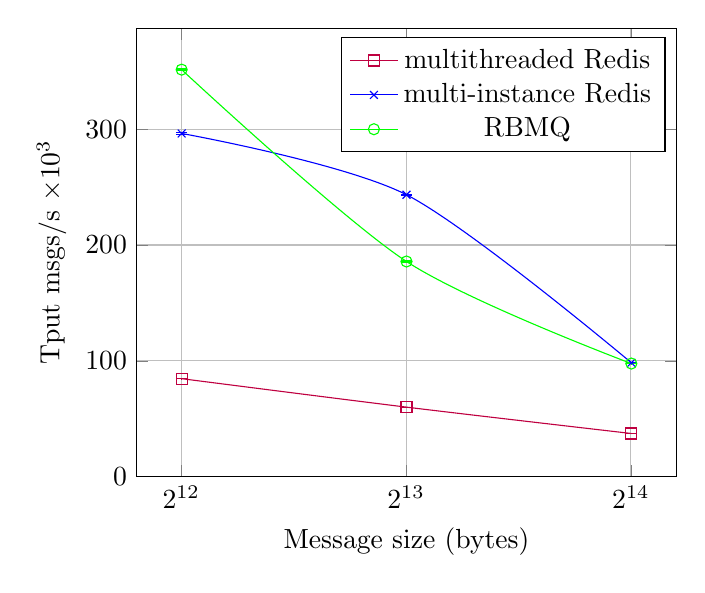
\begin{tikzpicture}
    \begin{axis}[
        xlabel=Message size (bytes),
        ylabel=Tput msgs/s $\times 10^3$,
        ymin=0,
        xmode=log, log basis x=2,
        enlarge x limits={0.1},
        grid=both,
    ]
      \addplot[smooth,color=purple,mark=square, error bars/.cd, y dir=both, y explicit]
        plot coordinates {
        (2^12,84.55088333333333333)+=(0,0.049754007439413488315)-=(0,0.049754007439413488315)
        (2^13,59.95895)+=(0,0.046476751628125782364)-=(0,0.046476751628125782364)
        (2^14,37.1893)+=(0,0.029682884535259879535)-=(0,0.029682884535259879535)
        };
        \addlegendentry{multithreaded Redis}
        
        \addplot[smooth,color=blue,mark=x, error bars/.cd, y dir=both, y explicit]
        plot coordinates {
            (2^12,296.39035)+=(0,0.75166904255183064437)-=(0,0.75166904255183064437)
            (2^13,243.43763333333303)+=(0,0.23271337431087902)-=(0,0.23271337431087902)
            (2^14,98.30368333333333333)+=(0,0.09571882038126067333)-=(0,0.09571882038126067333)
        };
        \addlegendentry{multi-instance Redis}

            \addplot[smooth,color=green,mark=o, error bars/.cd, y dir=both, y explicit]
        plot coordinates {
            (2^12,351.5146)+=(0,0.5670100402)-=(0,0.5669767068999999)
            (2^13,185.7915)+=(0,0.4200196067)-=(0,0.4199696067)
            (2^14,97.60255000000001)+=(0,0.09336207281)-=(0,0.09334540615)
        };
    \addlegendentry{RBMQ}
    \end{axis}
    \end{tikzpicture}
    \caption{Throughput of RBMQ broker, multithread Redis broker, multi-instance Redis broker with one subscriber and 95\% confidence intervals.}
    \label{fig:redis-multithread}
\end{figure}

\section{Using RocketBufs}
This section presents the observed challenges in adapting Redis, a popular MOM system, to run on top of RocketBufs.
To our knowledge, we are the first to provide feedback on the RocketBufs framework from the point of view of MOM developers.
We leave the job of performing this adaptation to future work.
 
The first challenge in adapting Redis to use Rocketbufs is the framework's lack of a C interface.
Redis is written in C, as too are many high performance applications as a result of the language's low overhead.
Such an interface might be helpful in attracting MOM system developers to make use of the framework.

%Section 3.2: "RocketBufs’ key APIs are asynchronous and completion events related to buffers are handled by registering callback functions."
The second challenge is RocketBufs' asynchronous API.
The RocketBufs interface is asynchronous and leaves completion events to be handled by a registered callback function.
Redis has a synchronous design such that each client is managed using a single thread of execution~\cite{redis-benchmark}.
Adapting Redis to use RocketBufs would potentially require adding thread synchronization structures. Asynchronous communication with clients would require reworking the system to handle communication failures occurring at any point after invocation.
Building or adapting an MOM system to use RocketBufs will require an asynchronous model, which tends to be more difficult to implement and reason about.
However, these concerns may apply primarily to Redis as many high performance applications already use an asynchronous model~\cite{10.1145/3359993.3366766}.

%Took this statement \& citation from conclusion of this paper: https://www4.cs.fau.de/Lehre/SS20/PS_KVBK/arbeiten/IO_Abstractions.pdf (I/O is faster than the OS)
%This transition may be accelerating with the release of Linux's new asynchronous I/O subsystem io\_uring, which has been steadily gaining support for a variety of operations~\cite{iouring}.

%may become more wide spread with the advent of Linux's \inlinecode{io\_uring} library, a rapidly growing
%Developers are interested in performing asynchronous I/O.
%A primary challenge that we see in attracting MOM designers design or redesign %their systems to use RocketBufs is the omnipresence of sockets used in %communicating over a network and the expansive set of libraries for using them.
%...
%Recently added Linux \inlinecode{io\_uring}


% I ADDED THE FUTURE WORK OF ADAPTING REDIS IN THE REDIS ADAPTATION SECTION
%\section{Discussion and Future Work}
%Here are the possible future works:\\
%- Finish the Redis implementation that uses RocketBufs
%\\
%- See how easy it will be to use RocketBufs with other MOM Systems such as %RBMQ
%
%\\
%\\- Utilize RocketBufs between servers not only between client and server
%%https://github.com/zzaoen/RdmaAcceleratingRedis


\section{Conclusion}
RocketBufs has the potential to enable MOM systems to quickly and easily make use of new and emerging network communication technologies, resulting in high-throughput and/or low latency network communication.
In our study, we reproduce a subset of the performance evaluations of RBMQ, a MOM system built on top of RocketBufs.
We are not able to validate the RocketBufs paper's claims about performance as a result of a lack of experimental artifacts.
While some challenges exist in building or adapting MOM systems to use RocketBufs, it is our belief that RocketBufs is a unique solution to an important problem.

%However, we find that RBMQ is able able to outperform a Redis broker with a more realistic configuration.
%Rocketbufs is different from anything else that 
%Better documentation of artifacts are required for other MOM systems to easily use Rocketbufs inorder to access modern datacenter technologies that it supports.
%Better documentation would have enabled us to reproduce matching results or draw better conclusions about our results. 

%- Rocketbufs is a unique framework
%- Our setup was similar to original experiment
%- Our results are not the same
%- Documentation would have helped

\section{Acknowledgments}

We would like to acknowledge Professor Brecht for his help and guidance in steering us toward a completed paper.
We would also like to acknowledge Lori Paniak for helping set up the machines for experimentation. Without his help, we would have no results.

{\footnotesize \bibliographystyle{acm} \bibliography{references.bib}}


\end{document}


% Note to self:
% From RocketBufs paper page 7 Section 4.2
% "Our Redis publishers and subscribers are implemented using the Redis-provided client library hiredis [56]. We run multiple Redis broker processes on the broker host in order to utilize all CPU cores, since each Redis broker process is single-threaded. For both Redis and RabbitMQ, we disable data persistence and event logging features to ensure that messages are handled in-memory only. We also tune both systems based on recommended best practices [53, 59] to optimize their messaging performance in our experiments."
% 53: !!!!IGNORE IT IS FOR RABBITMQ!!!! Pivotal. [n.d.]. Networking and RabbitMQ. https://www.rabbitmq.com/networking.html. Accessed Nov 17 2020
% 59: Redis. [n.d.]. Redis Documentation. https://redis.io/documentation. Accessed Nov 17 2020



% Notes on How to write a bad research paper:
% https://www.youtube.com/watch?v=K9BhQaOdtjs
% 1) Make sure to have something of value in the paper: a theory or experimental results
%  - no theorem and no experiments results in empty paper --> REJECTED
%
% 2) Don't just focus on solutions! Research needs to be solving a problem. Define the problem
% - define the problem
% - define its relevance: i.e.
%   - explain how others have tried to solve the problem (and presumably you have a better solution), or
%   - the problem has important to certain applications
%
% 3) Explain why the idea is novel! Emphasize what is new!
% - This is usually done by comparing to related work which is the existing work on the subject
%
% 4) Have a focus!
% - I'm interpreting this to mean that there's no clearly defined problem/goal, just a lot of little things that were done
% - this relates to the "story" previously discussed
% - make the connection clear between each steps you took
%
% 5) Have a message(?)
% - I think this is relevant to us
% - little unclear about this one as it's similar to (4)
% - avoid dumping everything in the paper and just focus on convey the message of the paper
% - don't tell the your story in conducting research
% - rejected for irrelevant details
%
% 6) Make sure the paper is understandable by a wider audience than your academic peers
% - carefully explain the ideas underlying problem and solution that is broadly understandable
%
% 7) Make sure that paper looks good (i.e., style, page limits, typos, references, etc)

% Plotted this, saw this, concluded this